\documentclass[11pt,compress,t,notes=noshow, xcolor=table]{beamer}


\input{../../style/preamble}
\input{../../latex-math/basic-math}
\input{../../latex-math/basic-ml}

\title{Optimization in Machine Learning}

\begin{document}

\titlemeta{% Chunk title (example: CART, Forests, Boosting, ...), can be empty
  First order methods
  }{% Lecture title  
  Comparison of first order methods
  }{% Relative path to title page image: Can be empty but must not start with slides/
  figure_man/linesearch.png
  }{
    \item Gradient Descent
    \item Stochastic Gradient Descent
    \item Momentum
    \item Step size decay
}


\begin{vbframe}{Comparison of first order methods}
Comparison of (S)GD, (S)GD + momentum, and (S)GD + momentum + step size control on simulated data. We do not use analytical solution on purpose although one exists:

\begin{itemize}
    \item Linear regression (squared loss) simulation $\bm{Y} = \bm{X}\thetav^{\ast} + \bm{\varepsilon}$ with $n=500$ samples and $p=11$ features, where $\thetav^{\ast}=(-5,-4,\ldots,4,5)^{\top}$, $\bm{\varepsilon} \sim \mathcal{N}(\bm{0}, \bm{I})$, and $\bm{X} \sim \mathcal{N}(\bm{0}, \Sigma)$ for $\Sigma=\bm{I}$ (indep. features) or $\Sigma_{i,j}=0.99^{|i-j|}$ (corr. features)
    \item Indep. features result in a condition number of $\approx 2.9$, whereas the corr. feature set-up produces a bad condition number of $\approx 600$
    \item We set the momentum parameter to $\texttt{momentum}=0.8$
    \item The step size $\alpha^{[t]}$ is decayed exponentially using deterministic schedule $\alpha^{[t]}=\alpha^{[0]} \cdot \texttt{decay}^{t/t_{\text{max}}}$ for $\texttt{decay}=0.1$
    \item For GD and SGD we use 3 step sizes each (low, medium, large). % to illustrate the effect of $\alpha$, $\texttt{momentum}$ and $\texttt{decay}$.
    \item ERM has unique global minimizer given by $\thetah = (\bm{X}^{\top}\bm{X})^{-1}\bm{X}^{\top} \bm{Y}$
    \item We also track the estimation error $\Vert \thetav - \thetav^{\ast} \Vert_2$
\end{itemize}

\end{vbframe}

%%%% GD linear

\begin{vbframe}{Lin-Reg (GD + med step size)}
\vspace{-0.4cm}
GD with medium $\alpha=2\cdot10^{-3}$ and indep. features:
\begin{figure}
            \includegraphics[width=0.8\textwidth]{slides/04-multivariate-first-order/figure_man/simu_linmod/GD_reg_med_lr_iters.pdf} \\
             \includegraphics[width=0.8\textwidth]{slides/04-multivariate-first-order/figure_man/simu_linmod/GD_reg_coef_med.pdf}\\
            \begin{footnotesize}
                Irreducible error due to additive noise is $\sigma=1$
            \end{footnotesize}
\end{figure}
Momentum accelerates optimization but all versions converge to global min. Decay slows down optimization slightly.
\end{vbframe}

\begin{vbframe}{Lin-Reg (GD + corr. features)}
\vspace{-0.4cm}
GD with medium $\alpha=2\cdot10^{-3}$ and bad conditioning (corr. features):
\begin{figure}
            \includegraphics[width=0.8\textwidth]{slides/04-multivariate-first-order/figure_man/simu_linmod/GD_reg_med_lr_corr_iters.pdf} \\
             \includegraphics[width=0.8\textwidth]{slides/04-multivariate-first-order/figure_man/simu_linmod/GD_reg_coef_med_corr.pdf}\\
            \begin{footnotesize}
                Irreducible error due to additive noise is $\sigma=1$
            \end{footnotesize}
\end{figure}
Only momentum  GD variant converges in $t_{\text{max}}$ iterations. Bad conditioning slows down optim severely!
\end{vbframe}


\begin{vbframe}{Lin-Reg (GD + small step size)}
\vspace{-0.4cm}
GD with (too small) $\alpha=3\cdot10^{-4}$ and indep. features:
\begin{figure}
            \includegraphics[width=0.8\textwidth]{slides/04-multivariate-first-order/figure_man/simu_linmod/GD_reg_small_lr_iters.pdf} \\
             \includegraphics[width=0.8\textwidth]{slides/04-multivariate-first-order/figure_man/simu_linmod/GD_reg_coef_small.pdf}\\
            \begin{footnotesize}
                Irreducible error due to additive noise is $\sigma=1$
            \end{footnotesize}
\end{figure}
Only momentum permits optim close to global min in $t_{\text{max}}=10000$ iters. Decay worsens performance as $\alpha$ was already too low.
\end{vbframe}

\begin{vbframe}{Lin-Reg (GD + large step size)}
\vspace{-0.5cm}
GD with large $\alpha=1.5$ and indep. features:
\begin{figure}
            \includegraphics[width=0.8\textwidth]{slides/04-multivariate-first-order/figure_man/simu_linmod/GD_reg_large_lr_iters.pdf} \\
             \includegraphics[width=0.7\textwidth]{slides/04-multivariate-first-order/figure_man/simu_linmod/GD_reg_coef_large.pdf}\\
            \begin{footnotesize}
                Irreducible error due to additive noise is $\sigma=1$
            \end{footnotesize}
\end{figure}
Super fast convergence in $<20$ steps. Decay here speeds up optim. Coefficients ``overshoot''+oscillate at beginning. Momentum variants become unstable.
\end{vbframe}


%%% SGD linear

\begin{vbframe}{Lin-Reg (SGD + med step size)}
\vspace{-0.4cm}
SGD with medium $\alpha=2\cdot10^{-3}$ and indep. features:
\begin{figure}
            \includegraphics[width=0.8\textwidth]{slides/04-multivariate-first-order/figure_man/simu_linmod/SGD_reg_med_lr_iters.pdf} \\
             \includegraphics[width=0.8\textwidth]{slides/04-multivariate-first-order/figure_man/simu_linmod/SGD_reg_coef_med.pdf}\\
            \begin{footnotesize}
                Irreducible error due to additive noise is $\sigma=1$
            \end{footnotesize}
\end{figure}
Momentum accelerates optim initially but eventually becomes worse. Momentum+decay is both fast and has small final error.
\end{vbframe}

\begin{vbframe}{Lin-Reg (SGD + corr. features)}
\vspace{-0.4cm}
SGD with medium $\alpha=2\cdot10^{-3}$ and bad conditioning (corr. features):
\begin{figure}
            \includegraphics[width=0.8\textwidth]{slides/04-multivariate-first-order/figure_man/simu_linmod/SGD_reg_med_lr_corr_iters.pdf} \\
             \includegraphics[width=0.8\textwidth]{slides/04-multivariate-first-order/figure_man/simu_linmod/SGD_reg_coef_med_corr.pdf}\\
            \begin{footnotesize}
                Irreducible error due to additive noise is $\sigma=1$
            \end{footnotesize}
\end{figure}
Bad conditioning slows down and destabilizes SGD optimization compared to indep. features. Momentum helps prevent this.
\end{vbframe}

\begin{vbframe}{Lin-Reg (SGD + small step size)}
\vspace{-0.4cm}
SGD with small $\alpha=3\cdot10^{-4}$ and indep. features:
\begin{figure}
            \includegraphics[width=0.8\textwidth]{slides/04-multivariate-first-order/figure_man/simu_linmod/SGD_reg_small_lr_iters.pdf} \\
             \includegraphics[width=0.8\textwidth]{slides/04-multivariate-first-order/figure_man/simu_linmod/SGD_reg_coef_small.pdf}\\
            \begin{footnotesize}
                Irreducible error due to additive noise is $\sigma=1$
            \end{footnotesize}
\end{figure}
Only momentum variants close to optimum in $t_{\text{max}}=10000$. Decay again worsens performance. Coef paths $\approx$ smooth due to small $\alpha$. 
\end{vbframe}


\begin{vbframe}{Lin-Reg (SGD + large step size)}
\vspace{-0.4cm}
SGD with large $\alpha=1 \cdot 10^{-2}$ and indep. features:
\begin{figure}
            \includegraphics[width=0.8\textwidth]{slides/04-multivariate-first-order/figure_man/simu_linmod/SGD_reg_large_lr_iters.pdf} \\
             \includegraphics[width=0.8\textwidth]{slides/04-multivariate-first-order/figure_man/simu_linmod/SGD_reg_coef_large.pdf}\\
            \begin{footnotesize}
                Irreducible error due to additive noise is $\sigma=1$
            \end{footnotesize}
\end{figure}
Highly noisy dynamics worsened by momentum. Step size decay necessary to eliminate noise toward end of training.
\end{vbframe}

\begin{vbframe}{Efficiently Solving OLS with QR Decomp.}

\textbf{QR Decomposition}:
\begin{itemize}
    \item Factorize \( \bm{X} \in \mathbb{R}^{n \times p} \) as \( \bm{X} = \bm{Q}\bm{R} \), where \( \bm{Q} \in \mathbb{R}^{n \times p} \) (economical form) and \( \bm{R} \in \mathbb{R}^{p \times p} \) is upper triangular.
    \item Purpose: Replace solving \( \bm{\thetah} = (\bm{X}^{\top} \bm{X})^{-1} \bm{X}^{\top} \bm{y} \) with a more numerically stable method by avoiding direct inversion.
    \item The QR decomposition can be computed using Gram-Schmidt orthogonalization or Householder transformations
\end{itemize}

\textbf{Steps}:
\begin{enumerate}
    \item Decompose \( \bm{X} \) into \( \bm{Q} \) and \( \bm{R} \).
    \item Compute \( \bm{Q}^{\top} \bm{y} \).
    \item Solve triangular system \( \bm{R} \bm{\thetah} = \bm{Q}^{\top} \bm{y} \) via \textbf{back substitution}.
\end{enumerate}

Why this system? Remember normal equation for least squares problem are $\bm{X}^{\top}\bm{X} \hat{\thetav} = \bm{X}^{\top}\bm{y}$. Now replace $\bm{X}=\bm{Q} \bm{R}$:

\begin{align*}
    \bm{X}^{\top}\bm{X} \hat{\thetav} = \bm{X}^{\top}\bm{y} &\iff \bm{R}^{\top}(\bm{Q}^{\top} \bm{Q}) \bm{R}^{\top} \hat{\thetav} = \bm{R}^{\top} \bm{Q}^{\top} \bm{y} \\
    \bm{R}^{\top}\bm{R} \hat{\thetav} = \bm{R}^{\top} \bm{Q}^{\top} \bm{y} & \iff \bm{R} \hat{\thetav} = \bm{Q}^{\top} \bm{y}\\
\end{align*}

After performing QR decomposition on \( \bm{X} \), we solve the triangular system:
\[
\bm{R} \bm{\thetah} = \bm{Q}^{\top} \bm{y},
\]
where:
\[
\bm{R} = \begin{bmatrix} 
r_{11} & r_{12} & \dots & r_{1p} \\ 
0 & r_{22} & \dots & r_{2p} \\ 
\vdots & \vdots & \ddots & \vdots \\ 
0 & 0 & \dots & r_{pp} 
\end{bmatrix}, \quad 
\bm{\thetah} = \begin{bmatrix} 
\thetah_1 \\ 
\thetah_2 \\ 
\vdots \\ 
\thetah_p 
\end{bmatrix}, \quad \bm{Q}^{\top} \bm{y} = \begin{bmatrix} 
b_1 \\ 
b_2 \\ 
\vdots \\ 
b_p 
\end{bmatrix}.
\]

\textbf{Steps for Back Substitution}:
\begin{enumerate}
    \item Start with the last equation (1 unknown):
          \[
          \thetah_p = \frac{b_p}{r_{pp}}.
          \]
    \item Move upwards to the \( (p-1) \)-th equation:
          \[
          \thetah_{p-1} = \frac{b_{p-1} - r_{p-1,p} \thetah_p}{r_{p-1,p-1}}.
          \]
    \item Continue this process up to the first row:
          \[
          \thetah_i = \frac{b_i - \sum_{j=i+1}^p r_{ij} \thetah_j}{r_{ii}} \quad \text{for each } i = p-1, \dots, 1.
          \]
\end{enumerate}

Back substitution leverages triangular structure of $\bm{R}$ to efficiently solve for $\bm{\thetah}$, moving from the last row upwards and substituting previously calculated values of $\bm{\thetah}$ as we go.

\end{vbframe}

\begin{comment}

\begin{vbframe}{Comparison of first order methods}
Comparison of (S)GD, (S)GD + momentum, and (S)GD + momentum + step size control on simulated data:

\begin{itemize}
    \item Logistic regression (cross-entropy loss) simulation also with $n=500$ samples and $p=11$ features, where $\thetav^{\ast}=(-5,-4,\ldots,4,5)^{\top}$ and $\bm{X} \sim \mathcal{N}(\bm{0}, \Sigma)$ for $\Sigma=\bm{I}$ (indep. features) or $\Sigma_{i,j}=0.99^{|i-j|}$ (corr. features)
    \item To simulate response, we set $y^{(i)} \sim \mathcal{B}(\pi^{(i)}), \pi^{(i)} = \frac{1}{1+e^{-(\bm{x}^{(i)})^{\top}\thetav^{\ast}}}$
    \item Indep. features again result in low condition number, whereas corr. features result in bad condition number
    \item We set the momentum parameter to $\texttt{momentum}=0.8$ and $\texttt{decay}=0.1$
    \item For GD and SGD we use 3 step sizes each (low, appropriate, large) to illustrate the effect of $\alpha$, $\texttt{momentum}$ and $\texttt{decay}$.
    \item ERM has unique global minimizer but no closed-form solution
    \item We also track the estimation error $\Vert \thetav - \thetav^{\ast} \Vert_2$
\end{itemize}

\end{vbframe}

%%% GD logistic


\begin{vbframe}{Log-Reg (GD + med step size)}
\vspace{-0.4cm}
GD with medium $\alpha=5\cdot10^{-2}$ and indep. features:
\begin{figure}
            \includegraphics[width=0.8\textwidth]{slides/04-multivariate-first-order/figure_man/simu_linmod/GD_log_med_lr_iters.pdf} \\
             \includegraphics[width=0.8\textwidth]{slides/04-multivariate-first-order/figure_man/simu_linmod/GD_log_coef_med.pdf}\\
            \begin{footnotesize}
                Dashed line in test loss indicates irreducible error due to $\sigma=1$
            \end{footnotesize}
\end{figure}
Momentum accelerates optimization while other versions still do not converge to global min. Decay slows down progress.
\end{vbframe}

\begin{vbframe}{Log-Reg (GD + corr. features)}
\vspace{-0.4cm}
GD with medium $\alpha=5\cdot10^{-2}$ and bad conditioning (corr. features):
\begin{figure}
            \includegraphics[width=0.8\textwidth]{slides/04-multivariate-first-order/figure_man/simu_linmod/GD_log_med_lr_corr_iters.pdf} \\
             \includegraphics[width=0.8\textwidth]{slides/04-multivariate-first-order/figure_man/simu_linmod/GD_log_coef_med_corr.pdf}\\
            \begin{footnotesize}
                Dashed line in test loss indicates irreducible error due to $\sigma=1$
            \end{footnotesize}
\end{figure}
Only GD with momentum converge in $t_{\text{max}}=10000$ iterations. Step size decay slows down optimization (non-convergence).
\end{vbframe}


\begin{vbframe}{Log-Reg (GD + small step size)}
\vspace{-0.4cm}
GD with small $\alpha=2\cdot10^{-3}$ and indep. features:
\begin{figure}
            \includegraphics[width=0.8\textwidth]{slides/04-multivariate-first-order/figure_man/simu_linmod/GD_log_small_lr_iters.pdf} \\
             \includegraphics[width=0.8\textwidth]{slides/04-multivariate-first-order/figure_man/simu_linmod/GD_log_coef_small.pdf}\\
            \begin{footnotesize}
                Dashed line in test loss indicates irreducible error due to $\sigma=1$
            \end{footnotesize}
\end{figure}
No method converges in $t_{\text{max}}=10000$, as small updates keep the process in high-error regions, accumulating error over time.
\end{vbframe}

\begin{vbframe}{Log-Reg (GD + large step size)}
\vspace{-0.5cm}
GD with large $\alpha=10$ and indep. features:
\begin{figure}
            \includegraphics[width=0.8\textwidth]{slides/04-multivariate-first-order/figure_man/simu_linmod/GD_log_large_lr_iters.pdf} \\
             \includegraphics[width=0.8\textwidth]{slides/04-multivariate-first-order/figure_man/simu_linmod/GD_log_coef_large.pdf}\\
            \begin{footnotesize}
                Dashed line in test loss indicates irreducible error due to $\sigma=1$
            \end{footnotesize}
\end{figure}
Super fast convergence for momentum around $30$ steps. Coefficient paths show ``overshooting'', while decay helps.
\end{vbframe}



%%% SGD logistic

\begin{vbframe}{Log-Reg (SGD + med step size)}
\vspace{-0.4cm}
SGD with medium $\alpha=5\cdot10^{-2}$ and indep. features:
\begin{figure}
            \includegraphics[width=0.8\textwidth]{slides/04-multivariate-first-order/figure_man/simu_linmod/SGD_log_med_lr_iters.pdf} \\
             \includegraphics[width=0.8\textwidth]{slides/04-multivariate-first-order/figure_man/simu_linmod/SGD_log_coef_med.pdf}\\
            \begin{footnotesize}
                Dashed line in test loss indicates irreducible error due to $\sigma=1$
            \end{footnotesize}
\end{figure}
Momentum accelerates optim but all variants except decay converge. Coef paths slightly jittered.
\end{vbframe}

\begin{vbframe}{Log-Reg (SGD + corr. features)}
\vspace{-0.4cm}
SGD with medium $\alpha=5\cdot10^{-2}$ and bad conditioning (corr. features):
\begin{figure}
            \includegraphics[width=0.8\textwidth]{slides/04-multivariate-first-order/figure_man/simu_linmod/SGD_log_med_lr_corr_iters.pdf} \\
             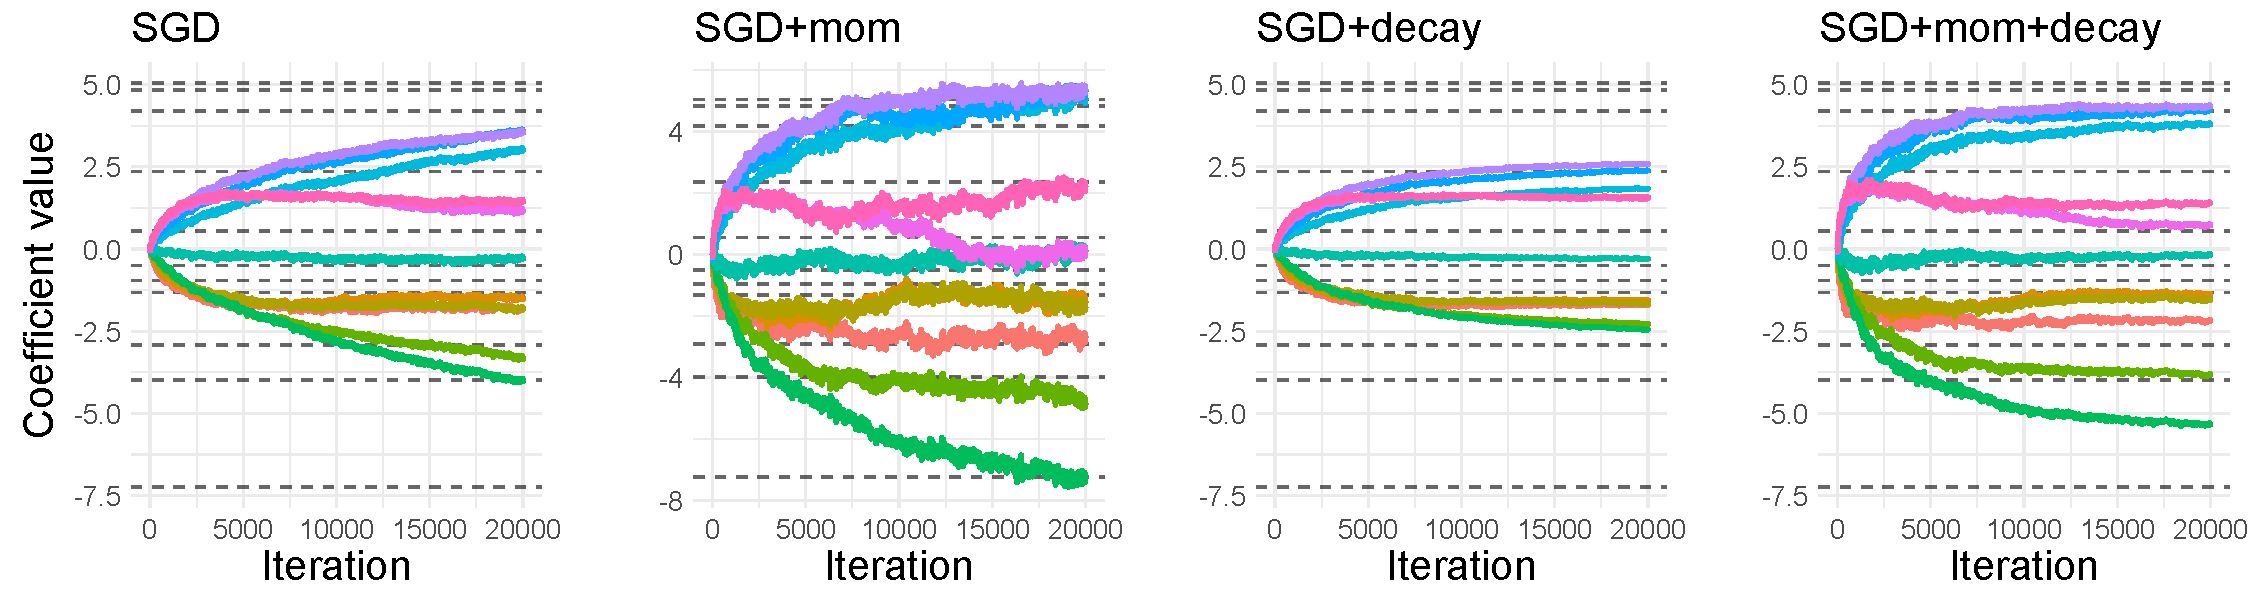
\includegraphics[width=0.8\textwidth]{slides/04-multivariate-first-order/figure_man/simu_linmod/SGD_log_coef_med_corr.pdf}\\
            \begin{footnotesize}
                Dashed line in test loss indicates irreducible error due to $\sigma=1$
            \end{footnotesize}
\end{figure}
Only SGD and SGD+mom converge in $t_{\text{max}}=10000$. Decay slows down while momentum accelerates optim.
\end{vbframe}


\begin{vbframe}{Log-Reg (SGD + small step size)}
\vspace{-0.4cm}
SGD with small $\alpha=3\cdot10^{-4}$ and indep. features:
\begin{figure}
            \includegraphics[width=0.8\textwidth]{slides/04-multivariate-first-order/figure_man/simu_linmod/SGD_log_small_lr_iters.pdf} \\
             \includegraphics[width=0.8\textwidth]{slides/04-multivariate-first-order/figure_man/simu_linmod/SGD_log_coef_small.pdf}\\
            \begin{footnotesize}
                Dashed line in test loss indicates irreducible error due to $\sigma=1$
            \end{footnotesize}
\end{figure}
No method converges since lr is too small. Decay makes it even worse. 
\end{vbframe}


\begin{vbframe}{Log-Reg (SGD + large step size)}
\vspace{-0.4cm}
SGD with large $\alpha=1.5$ and indep. features:
\begin{figure}
            \includegraphics[width=0.8\textwidth]{slides/04-multivariate-first-order/figure_man/simu_linmod/SGD_log_large_lr_iters.pdf} \\
             \includegraphics[width=0.8\textwidth]{slides/04-multivariate-first-order/figure_man/simu_linmod/SGD_log_coef_large.pdf}\\
            \begin{footnotesize}
                Dashed line in test loss indicates irreducible error due to $\sigma=1$
            \end{footnotesize}
\end{figure}
Only variants with simple decay converge, others overshoot severely. Loss and coef paths very noisy.
\end{vbframe}

\end{comment}

\endlecture
\end{document}

%%% 



%% 
